% ===================================================== %
% =========== BSL INTERN MANUAL ======================= %
% ===================================================== %

% Mathieu Barbin, 2nd semester 2009

\documentclass[10pt]{article}

% Pour les accents dans les fichiers
\usepackage[T1]{fontenc}        % Codage des fontes
\usepackage[latin1]{inputenc}   % Codage du fichier
\usepackage[english]{babel}    % For english
\usepackage[colorlinks = true, urlcolor = magenta]{hyperref} % Utilisation de HyperTex
% Packages AMS très utiles
\usepackage{amssymb,amsfonts,amsthm,amsmath,graphicx}

\title{Opa and Qml (Bypass) Standard Library - Internal Manual}
\date{Version 1.1}
\author{Mathieu Barbin - Mehdi Bouaziz}

% Définitions d'environements

\newtheorem{syntax}{Syntax}
\newtheorem{example}{Example}
\newtheorem{remark}{Remark}
\newtheorem{convention}{Convention}
\newtheorem{code}{Code}

\begin{document}
\maketitle
%% \begin{figure}[!h]
%% \begin{center}
%%     \includegraphics[scale=0.2]{beboplogo.eps}
%% \end{center}
%%   \end{figure}
\tableofcontents

\part{Introduction}
\section{Please read this just before reading anything else}
If you're reading it, you probably {\bf{need informations}} about the way {\bf{libbsl}} works. \\
So, by browsing this manual, if you {\bf{don't find}} an appropriate answer to your question, please feel totally free to {\bf{add any remark or comlement to the source of this manual}} (see the source {\bf{bslmanual.tex}} in {\textit{libqml.git/libqml/libbsl/manual/}}) (and by the way, thank you for your contribution in correcting the bad english you will find in this little manual...).\\
\paragraph{FAQ}
If you really need an information and you don't find it, please {\bf{go to the FAQ}}, and write your question there.\\
It will be a {\bf{gain of time}} for the whole MLstate team ! Thank you, and enjoy your bsl-using time !
\paragraph{Quiz}
After reading the manual, you can go to the bsl-quiz, and try to see you score !
\section{What is this document ?}
This manual is an {\bf{intern document for MLstate's team}} to expose the main ideas implemented in the {\bf{libbsl.cmxa}}. It is made in the hope that : 
\begin{enumerate}
\item it will facilite the integration of the bsl in the compilation-chain (Louis, Mikolaj, Geoffroy)
\item that could help the library-guy to make his job (Nicolas)
\end{enumerate}
This document is not a documentation of the runtime standard library for users of mlstate technologies !
\section{Code documentation}
The main modules-API are in the documented \textit{.mli} files. You can also find the ocamldoc generated pages in {\textit{libqml.git/libqml/libbsl/Register/html}}.

\section{What is the bsl ?}
\subsection{Main Ideas}
{\bf{bsl}} means {\textit{Bypass Standard Library}}, so you got it, this lib is about {\textit{the binding of bypass functions}}.\\
 The main point is that the solution of having raw code in the bypass, like it was done until now, is complex to deal at different levels, from {\bf{compilers}} to {\bf{verification tools}}, and of course for {\bf{interpreters}}. \\
~\\
The {\bf{\textit{libbsl}}} proposes a restriction mechanism based on {\bf{keys instead of raw code}}, and make a {\bf{transtyping code generation}}. \\
~\\
{\bf{From implementations files in c, ml, js, + mixed code in opa, qml + your representation of type in your compiler or interpreter}}
\begin{itemize}
\item we'll build for you a lib in which you can access all the bypass-functions with good {\bf{introspection facilities}}, and with the possibility (with a specialized BSL) of having the generated functions working directly on your representation of types 
\item we will generate opainit, qmlinit in syntax and ast format containing all {\bf{bypass binding definitions}}, {\bf{merged with the hand-written mlstate-library-code}}
\end{itemize}
All the mlstate init code (opaini, qmlinit) is fully shared for all the applications (compilers, interpreters, slicers, analysers, etc...)\\
The bypass introduced in the implementation-files in ml of the {\bf{\textit{libbsl}}} are shared to be used in the qmltop-level, or in the qml2ocaml compiler.\\
For more details about the building process, please go to the part : {\textit{Libslbuilder : bslregister}} 

\subsection{Bypass Introspection}
As written in the documentation of ocaml-module Dynlink,  
\begin{quote}
No facilities are provided to access value names defined by the unit
\end{quote}
However, this mechanism is too specific to be shared between all the sources in the bsl (ml,c, js, qml, opa).\\
So we have here something more extensible, based on a main possibility of {\bf{implementation-registering}}\\
With {\bf{introspection}} we mean the possibility in your compiler to work on a dynamic map containing all the bypass functions. The main algorithm is the following :
\begin{enumerate}
  \item I meet a bypass-key in my ast
  \item I look in my bypass map, and I get all informations I need (In what languages is implemented this function, in what files, what is its type, ...)
  \item I use these informations to continue my job
\end{enumerate} 
To have access to the bsl, just link your application with the {\bf{libbsl.cmxa}}. A bonus introspection is given for interpreters :
\begin{quote}
in case of a ml-implementation, you'll get a pointer to the function {\bf{Obj.t}}
\end{quote}

\subsection{Unified Opa/Qml Standard Library}
A functionality with the {\bf{\textit{libbsl}}}, is that you don't need at any time to write any code looking like :
\begin{verbatim}
val abs = %%abs%% : int64 -> int64
val ^ = %%^%% : string -> string -> string
val compare = %%compare%% : 'a -> 'a -> int64
...
\end{verbatim}
or worth, 
\begin{verbatim}
let qmlinit = "
val abs = %%abs%% : int64 -> int64
val ^ = %%^%% : string -> string -> string
val compare = %%compare%% : 'a -> 'a -> int64
...
"
\end{verbatim}
this both kind of code are generated from directives and formats in your opa/qml code (see the following example). \\
~\\
BTW, there is also a {\bf{meta-ast code production in ocaml}}, then the ast of qmlinit and opanit could be {\bf{a const of type Ast}} in a generated ml code included in the {\bf{\textit{libbsl}}}, compiled.\\
~\\
In the opa and qml side, you can also write mixed code :
\begin{verbatim}
(* This is bslinit.qml *)
(* definition of format for qml syntax *)
##format import-module "let #n = %%#k%% : #t in"
##format bind "#n = #n" " ; "

(* let's go ! *)
(* import all top-level bypass from bypervasives *)
##include "val #n = %%#k%% : #t" bypervasives

 type qmltime = { h : int; m : int; s : int }  

 val time = 
   (* using the format to include function definitions from bypass module time *)
   ##include import-module time  
   let qmlt () =    
     let t = now () in 
     { h = hour t; m = min t; s = sec t } in 
   {  
    (* add the bypass functions to this record *)
    ##include bind time        
    ; qmlt = qmlt : unit -> qmltime } 
\end{verbatim}
or, in opa :
\begin{verbatim}
string =
  (* preprocess inclusion of bypass module string *)
  ##include "#n = %%#k%% : #t;" string
   
  get_from_end(s, n) = get(s, length(s) - n - 1);
	
  string_of_chars( l ) =   
    s = string_create( list.length( l) );
    !list.fold_left( (acc,x ->  !string_unsafe_set(s,acc,x) ; acc + 1), 0, l ) ;
    s
  ;

  {
    ##include bind string
    string_of_chars = string_or_chars
  }
\end{verbatim}

~\\
To see what is generated from these directives, go to section \emph{Testing the bslpreprocessor directives}.
~\\

You can find the documentation of directives {\bf{include and format}} in the part : {\bf{Linking of bypass functions in UnifOpa/Qml lib}}
Essentially, remember that 3 informations are essentials in a bypass, its {\bf{name}}, its {\bf{key}}, and its {\bf{type}}, you can acces them in a format with  {\bf{\#n, \#k, \#t}} 



\part{General use of the standard-bsl}
\section{Installing the libbsl}
\subsection{Git repository and depends}
The {\bf{\textit{libbsl}}} is in {\textit{libqml.git/libqml/libbsl/}}. It depends on {\bf{libqml.cmxa, libqmlcompil.cmxa, and more recently on db3.cmxa}} . \\
The installation requires the same ENV var as usual, {\bf{MLSTATELIBS}}, {\bf{TRX}}, ...\\
To have a {\bf{\textit{libbsl}}} working properly, you should add {\bf{MLSTATELIBS/bin}} to your PATH. 
\subsection{The installer is an ocamlbuild}
Since Louis has made the new build refactoring, the compilation/installation of libbsl is done by ocamlbuild/mkinstall.sh
\subsection{What is lib runtime ?}
A good target is to try to {\bf{reduce the size}} of the {\bf{binary of servers}} produced with {\textit{MLstate technology}}. The server don't need all the {\bf{libbsl}}. (for example, what will the server do with the introspection functions ?) \\
~\\
The ml-runtime bsl, {\textit{see the Makefile-variable {\bf{LIBBSLMLRUNTIME}}}}, is just what is needed at runtime, and must be linked to the {\bf{ocaml generated files (servers)}} in a {\bf{qml2ocaml process}}. \\
~\\
The same thing is possible in C and JS, (with js, it is the concatenation of all the code to send to the clients)
~\\
the lib {\bf{libbsl.cmxa}} is the complete lib that you need to link with your compiler. It contains the runtime lib.

\section{Standard Types}
The {\bf{Standard Types}} are the types allowed for bypass functions. This type algebra is {\bf{reduced compared with the qml type algebra}}, because the standard types are the {\bf{type interface}} 
between all the bypass languages and mlstate-languages (for example, no overload in bypass, etc.) and because
every standard type will require some work, mainly type-transcription (qml <-> host language representation). 
~\\
The {\bf{\textit{libbsl}}} contains specific tools working on this type algebra, including {\bf{binding functions with the algebra of the TypeChecker of libqml}}, etc. They are grouped together in the module {\textit{\bf{StandardType}}}. ~\\
\subsection{Extern types}
Notice the possibility of {\bf{extern-types}} : any value of such a type {\bf{does not have a representation in qml}}, and you provide in the bypass-library an implementation for a qml-API working on this type.\\
This is sensibly the same thing as {\bf{abstract types}}, but the abstract types in qml {\bf{do have a qml-implementation}}, so we decide to call these types {\bf{extern}} in the algebra to avoid this confusion, but actually, in qml and opa, the syntax to introduce an extern type is 
\begin{verbatim}
type toto = abstract
\end{verbatim}
so, be careful with these 2 different concepts.
\subsection{Interfaces between bypass-languages}
\paragraph{not(Extern)}
We denote by $n$ the number of bypass-languages, and by $t$ the number of standard types.\\
As long as a standard type is not extern, it has a representation in qml, so the interface between languages is assured by passing by the qml representation (star graph * with qml in the middle : just a couple of transcription functions for each standard type, and for each language, from host to qml); it is $2*n*t$ functions.\\
\paragraph{Extern}
An extern type can be implemented just in {\bf{one or more}} bypass-language, and in this case, the API must be {\bf{unified}}. Then comes the problem of {\bf{value-passing}} between bypass languages, because they may have different representations in each bypass-lang. \\
To avoid a bad combinatory explosion of work $n*(n-1)*t$ for the mlstate team, and in order to have {\bf{communication between languages}} (practically between
a {\bf{client language}} (JS) and a {\bf{server language}} (ML or C)), we need a {\bf{common
representation}} between these languages. This cannot be a qml type, so this is done by {\bf{serialization}}.
\subsection{Common JSON value-serialization}
Serialization and unserialization calls will be written by compilers guys.
If serialization or unserialization is not specified for an extern type,
it won't be possible to transfer data of this type between client and server (also note that with the libbsl, the slicer will introspect this information).\\

For example, if you have a type time\_t on which you have functions implemented in both JS and ML :
\begin{itemize}
\item In ML, you have
\begin{verbatim}
type time_t = float
\end{verbatim}
\item and in JS you use the Date object.
\end{itemize}
If you choose to use the json string transcription of the float version for the common representation you will need :
\begin{verbatim}
##import JSON
##register time_t_serialize \ JSON.of_float : extern time_t -> json 
##register time_t_unserialize \ JSON.to_float : json -> extern time_t
\end{verbatim}
and
\begin{verbatim}
##register time_t_serialize : extern time_t -> json
function time_t_serialize(t) {
	 return (t.getTime() / 1000).toString();
}
##register time_t_unserialize : json -> extern time_t 
function time_t_unserialize(f) {
	 var t = new Date();
	 t.setTime(eval(f) * 1000);
	 return t;
}
\end{verbatim}
For parametric extern types, see this example :
\begin{verbatim}
type ('a, 'b) t = ...

##register t_serialize : ('a -> json) -> ('b -> json) -> extern 'a 'b t -> json 
##register t_unserialize : (json -> 'a) -> (json -> 'b) -> json -> extern 'a 'b t
\end{verbatim}
Please, by keeping the naming convention typename\_serialize and typename\_unserialize, you will simplify the life of programmers.\\
This is useful if you want the serialize and unserialize functions to be part of the module Typename.
\subsection{Some problems about memory allocation / GC with LLVM}
When you add c functions in the libbsl, there is some problem with the type string which doesn't exist in c. Then when you have :
\begin{verbatim}
##register myfunction : string -> string
##args(a)
\end{verbatim}
The variables a has the type char*, then you can use string but it can have memory leak\ldots
  
\section{Dynamic Introspection}
\subsection{Bypass types and implementation}
From a {\bf{normalized key}}, you get a ByPass.t, and you can use the BSL API to access all the informations you need in your activity {\bf{cf. libBSL.mli}}:
\begin{itemize}
\item type
\item differents implementations (what language, where, ...)
\item if necessary, get a ocaml pointer on the implementation if it is in ocaml (useful for {\textit{qmltop}})
\item if you are using a {\bf{specialized bsl in a compiler}}, you will get the {\textit{bsl-generated-translation}} of the {\textit{origin-implementation}}, {\bf{\textit{working directly}}} on your {\textit{runtime-value-representation}}  
\end{itemize}

\subsection{Languages-restricted initial opa or qml code}
In the {\bf{ByPassMap API}}, there are some functions to filter bypass functions. Depending on {\bf{the kind of your application}}, you cannot use any bypass-language. For example, {\bf{qmltop}} cannot use {\bf{javascript functions}}, {\bf{qml2llvm}} is not interested in bypass functions implemented in ocaml only, ...\\
~\\
With a simple dependency calculus processing on {\bf{qmlinit and opainit}} functions and modules, your can regenerate the part of the mlstate initial lib, specialized for your application, filtering everything that you won't or cannot use.

\section{Libslbuilder : bslregister}
The application blsregister is the main builder of the libbsl :
\begin{figure}[!h]
  \begin{center}
    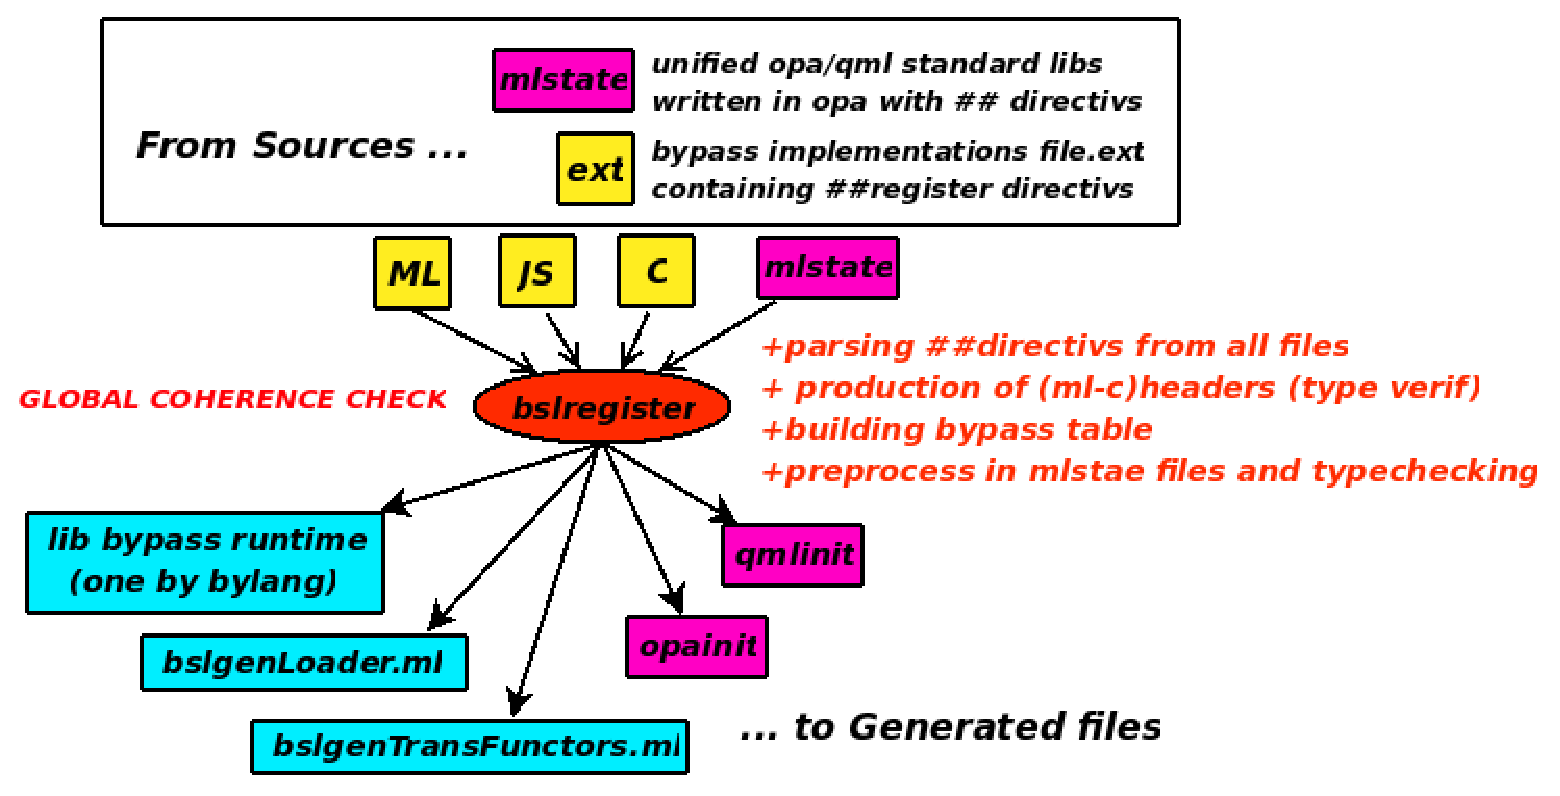
\includegraphics[scale=0.2]{bslregister.eps}
  \end{center}
\end{figure}

\subsection{Coherence and types verification}
\paragraph{Bypass}
All the directives {\bf{\#\#register}} give all the needed information to check that in each language, the definitions are coherent. The main point is : \begin{quote}How to verify during this building (and not later, at compile time, or at runtime) that the bypass-implementation have really the type defined in the register directive ?\end{quote}
A first answer is 
\begin{quote} 
{\bf{the bsl is an intern library, and our team does a very good job}}. Note that the directives are written just where the function is implemented, so we see both of them when we're adding an implementation in a bypass file.
\end{quote}
But {\bf{bslregister's}} answer is the following :
\begin{quote}
Because wo {\bf{do not want to analyse}} the bypass files (written in c, ml, js), we produce a {\bf{main header}} for each runtime library {\bf{\{mli, h, js?\}}} using the type definitions introduced with the directives. Then, we let {\bf{gcc}} and {\bf{ocamlopt}} do the job, at {\bf{libbsl-compile-time}}.
\end{quote}
\paragraph{Mlstate safe init code}
After preprocessing, the mlstate init code (opa, qml), is {\bf{parsed}}, {\bf{typed}}, and every error will be reported, and provoques a {\bf{failed libbsl building process}}. At this time, we produce the {\bf{ocaml-code}} representing the {\bf{ast}} value of this mlstate-init-code, and it is produced in the {\bf{loader}} (see the generated {\bf{BslgenLoader}}) as a {\bf{builtin static constant}} of type {\bf{Ast.code}} in the {\bf{libbsl}} 


\section{The introspection tool bslbrowser}
After the {\bf{make install}}, and checking that {\bf{\$MLSTATELIBS/bin/}} is in your {\bf{PATH}}, try it !
\begin{verbatim}
you@somewhere:~$ bslbrowser
bslbrowser version 1.1 : (c) 2009 MLstate {m&m}
bslbrowser:/$ help
Testing bsl-preprocessor :
	##format <name> <fmt> <sep>?   : bslregister new format definition (see manual)
	##include <fmt> <sep>? link    : bslregister include (#k : key - #n : name - #t : type)
	##include-type <regexp>        : bslregister type definition inclusion
	##module <name>                : bslregister new module definition
	##endmodule , ##import <name>
	##register key \ impl : type   : bslregister main directive
	##record name = typedef        : definition of record type

bslbrowser command help :
	cd .. / ~ / module          : navigation in modules
	ls [-t -d -m] <regexp>      : see contains of current location
	pwd                         : see current location
	help                        : plot this help menu
	types [ -lang ]             : see bsl types in differents format
	find [-t -bypass] <regexp>  : find module / or function in lib
	key [-t] <regexp>           : lookup in bsl keys
	bypass [-t] <regexp>        : same as key
	option -t                   : match types, not names
	option -d -m                : show modules only
	regexp                      : show ocaml manual of regexp
	com | unix                  : pipe (you can use grep or cat)
	quit or exit                : quit bslbrowser
bslbrowser:/$ 
\end{verbatim}
The bslbrower has been implemented as {\bf{a tester of the building process of libbsl}}, and because it could be used as a {\bf{code sample}}, which you can look into if you need to use the {\bf{libbsl}} API.\\
By the way, it also can be used as a {\bf{browser}} ! (and can be useful to quick-search in command line)
\begin{verbatim}
bslbrowser:/$ find _of 
+ in bypervasives :
    string_of_float    : float -> string {ml:top, ml}
    float_of_int       : int64 -> float {ml:top, ml}
    string_of_char     : char -> string {ml:top, ml}
    int_of_char        : char -> int64 {ml:top, ml}
    char_of_int        : int64 -> char {ml:top, ml}
    string_of_int      : int64 -> string {ml:top, ml}
    float_of_string    : string -> float option {ml:top, ml}
    int_of_string      : string -> int64 option {ml:top, ml}
    int_of_float       : float -> int64 {ml:top, ml}
\end{verbatim}
\subsection{Testing the bslpreprocessor directives}
If you implement something in the unified library (in opa, or qml initial files), you can test your inclusion format in the browser, it will print
the same output as the preprocessor will insert in your file :
\begin{verbatim}
bslbrowser:/$ ##format simple "name : #n -- key : #k -- typ : #t"
bslbrowser:/$ ##include simple bypervasives/string_of_int
name : string_of_int -- key : string_of_int -- typ : int64 -> string
bslbrowser:/$ ##include "val #n = %%#k%% : #t"  bypervasives    
val add_float = %%add_float%% : float -> float -> float
val abs = %%abs%% : int64 -> int64
val ^ = %%^%% : string -> string -> string
val mult_float = %%mult_float%% : float -> float -> float
val lte = %%lte%% : 'a -> 'a -> bool
val div_int = %%div_int%% : int64 -> int64 -> int64
val compare = %%compare%% : 'a -> 'a -> int64
val string_uppercase = %%string_uppercase%% : string -> string
val gte = %%gte%% : 'a -> 'a -> bool
....
\end{verbatim}

\section{Minimal ocaml-code using the standard libbsl}
\subsection{Load the bypass, and build the map}
For a simple use of the bsl, you will use the default bsl-module called {\bf{BSL}}. 
\begin{enumerate}
\item {\bf{load the bypass}} : has side-effect on the {\bf{\textit{RegisterTable}}}
\item {\bf{build the map}} : returns a functional structure containing the current state of the table
\item {\bf{use the map, with the API !}} : see mli files, ocamlbrowser, ... 
\end{enumerate}
\subsection{Sample : hello-libbsl}
{\bf{file : minimal.ml}} (from {\textit{libqml.git/libqml/libbsl/samples}}) :
\begin{verbatim}
open LibBSL

let _ =
  print_endline "minimal code sample using the libbsl";
  print_endline "loading the bsl";
  BSL.RegisterInterface.dynload BslgenLoader.dynloader;
  print_endline "building the functionnal structure";
  let bymap = BSL.RegisterTable.build_bypass_map () in
  print_endline "using the map :";
  BSL.ByPassMap.iter (fun k b -> print_endline (Printf.sprintf "key:\"%s\" -- type:\"%s\"" 
        (BslKey.to_string k) (StandardType.to_string (BSL.ByPass.definition_type b)))) bymap
\end{verbatim}
\subsection{Sample : hello-makefile}
To compile your application, you need to link it with the dependencies libs, as follows :
\begin{verbatim}
# Compiling a project using libbsl :
OCAMLOPT=ocamlopt.opt
LINKLIB = -thread -I +zip -I $(MLSTATELIBS)/libqml -I $(MLSTATELIBS)/libqmlcompil \
  -I $(MLSTATELIBS)/db3 -I $(MLSTATELIBS)/libbsl
XA = unix.cmxa threads.cmxa str.cmxa zip.cmxa libqml.cmxa libqmlcompil.cmxa \
  db3.cmxa libbsl.cmxa

minimal : minimal.ml
    $(OCAMLOPT) $(LINKLIB) $(XA) $^ -o $@
\end{verbatim}

\part{Specific use of the bsl for compilers and interpreters}
\section{Generation of transtyping functions for your runtime typed-representation of values}
The introspection functionality is 
\section{I am a qml2ocaml compiler, written in ocaml}
\section{I am a qmltoplevel, written in ocaml}
\section{I am a qml2llvm compiler, written in ocaml}

\part{Extending the bsl and writing new libraries}
\section{Introduction}
This section is here to help you if you want to write new libraries using the libbsl.\\
Note that there are 2 ways to build new libraries using {\bf{bslregister}} :
\begin{enumerate}
\item work directly in the libbsl repository, and add you work into the main libbsl.cmxa
\item use the bootstrap version of {\bf{bslregister}}, and build a {\textit{local}} library that won't be integrated in the libbsl.cmxa
\end{enumerate} 
An other possibility is also to test your work in a local folder, using the 2nd possibility, and after that integrate your work to the main libbsl. Note finally that with {\bf{git}}, you don't really need to be so careful, because you can just work on a local branch, adding your lib to the main libbsl.\\
So, it will mainly depend on the kind of your lib, if it is a very specific one, (like the {\textit{khipik-library}}, which is also built with {\bf{bslregister}}, but not added to libbsl.cmxa) or if your lib is written to be added to the {\bf{mlstate stdlib}} (like list, map, etc...)
\subsection{Architecture of stdlib and keys-normalization}
All the init code is organised in modules, like it is done in ocaml stdlib. The names of all bypass are normalized: lowercased, and replacing the '.' split between modules by '\_'. For example, {\bf{''ByPervasives.+.''}} will be normalized as {\bf{''bypervasives\_+.''}}. The same normalization is done for {\bf{type identifiers}}. 
\subsection{Guidelines}
To respect the coherence of the stdlib, please try to follow these simple guidelines:
\begin{itemize}
  \item the module names are lowercased in qml
  \item split the implementation in one file by module (in each bypass-lang), where the name of the file is the qml-name of the module
  \item if it makes sense, try to call the main type of a module {\bf{t}}
  \item try to keep a certain coherence between the architecture of the code in the bypass-language and the qml/opa binding code (e.g in ocaml with module architecture)
  \item try to think about the serialization of extern-types as soon as possible
  \item check the type inference of the mlstate part of your lib in the generated interface files (.qmli, .opai)
  \item test the inclusion of your lib during the libbsl building process (bslbrowser, qmltop, qml2ocaml, etc...)
  \item replace the return type of any function which may fail by raising an exception, by an option type
\end{itemize}

\section{Implementation of Bypass}


\section{Unified Opa/Qml Standard Library}
\subsection{Linking of bypass functions in UnifOpa/Qml lib}
\paragraph{directive include}
The directive include is used as a macro-processor of qml or opa code, introducing {\bf{binding-definitions}} between {\textit{\bf{qml-opa-function-names}}}, and {\bf{\textit{bypass-function-keys}}}.\\
For example, in {\textit{qml-init}}, where you used to write :
\begin{verbatim}
val +. = %%+.%% : float -> float -> float
val -. = %%-.%% : float -> float -> float
....
\end{verbatim}
You will write :
\begin{verbatim}
##include "val #n = %%#k%% : #t" bypervasives
\end{verbatim}
The directive {\textit{\bf{\#\#include}}} takes a {\textit{format}} as argument (and an optionnal {\textit{separator}}), containing the following links :
\begin{enumerate}
  \item {\bf{\#n}} : the qml-opa name of the bypass, declared with register : \verb�##register name \ impl�
  \item {\bf{\#k}} : the generated uniq-bsl-key
  \item {\bf{\#t}} : the definition type, printed in the syntax depending on the extension of the preprocessed file
  \item {\bf{\#m}} : the name of the module (for module-format only)
\end{enumerate}

\subsection{Recursive formats, definitions of a new format}
If you feel like writing here more explanations about the use of formats, please, make your way until the bslmanual.tex ;) \\
%% oh! you realy did! thank you ;) 
%% np :)
Other way : you can test it under {\bf{bslbrowser}}. For recursive formats : see the following syntax  
\begin{itemize}
  \item iterator : {\bf{\#\{module-rule, function-rule\}}} : use it to descend into a module and iter on its content
  \item rec :{\bf{\#rec}} : use it to specify as the module-rule the format itself for a deep-descend 
\end{itemize}
A few examples :
\begin{verbatim}
##format function "val #n = %%#k%% : #t"
##format functions "let #n = %%#k%% : #t in"
##format bind-module "#m = #m"
##format bind "#n = #n" " ; "
##format sub-module "let #m = \n#{#rec, functions}\n { #{bind-module, bind} } in" 
##format module "val #m = \n#{ sub-module, functions }\n  { #{bind-module bind} }"
##format pervasives "#{function}"
##format plot_hierarchy "module #m #{#rec}"
\end{verbatim}

\section{Complete use of the application bslregister}
The application {\bf{bslregister}} is the bypass librairies builder. This application has a first instance which is compiled before the main libbsl build process. This tool can be bootstrapped.

It is installed in {\textit{\$MLSTATELIBS/bin}} during the installation of libbsl.  
\subsection{For c files}
You can read this for all languages but it can be not exactly the same.\\
First for a c functions you must go in the folder {\textit{libqml.git/libqml/libbsl/cbsl/}}\\
There is a file {\textit{libqml.git/libqml/libbsl/cbsl/bsl-sources}}\\
In this file you must write your c file with one file on one line.\\
Examples :\\
\begin{verbatim}
include.c
cbsl.c
byPervasives.c
time.c
bool.c
byString.c
byStdio.c
char.c
\end{verbatim}
The include.c files just keep the c library call, all the other files contain functions.\\
When you add a function you must use a specific syntax for bslregister.\\
\\
First line :
\begin{verbatim}
##register myfunctions : int64 -> int64
\end{verbatim} 
Here the functions will be named \verb�thefile_myfunctions� if this function is in the file named thefile.c.\\
\\
Second line :
\begin{verbatim}
##args(u)
\end{verbatim}
This line will create automatically the header of your function which is here :\\
\begin{verbatim}
long long int thefile_myfunctions(long long int u)
\end{verbatim}

And after you have just to write your function.
 

\subsection{Syntax of directives}
\subsection{Using the command line tool}

\section{Complete-Example of libbsl-extension}
We will follow here the complete procedure by adding a new module {\bf{char}} in the stdlib (note that when you will read this, the module will already be added, because we really do it by writing this part of the manual).\\
Ok, we begin this example, let's see the date of the system :
\begin{verbatim}
samedi 2 mai 2009, 16:39:32 (UTC+0100)
\end{verbatim}

\subsection{Implementation file}
We will start with a ocaml implementation file, so we edit a new file in the libqml repository, at the right location (where all the ml-implementations are : {\textit{libqml.git/libqml/libbsl/mlbsl/char.ml}}).\\
We want to see which functions could be added in this module. So, we open a ocamlbrowser, and let's see the module char :
\begin{verbatim}
Char 
  type t = char
  chr : int -> char
  unsafe_chr : int -> char
  code : char -> int
  compare : t -> t -> int
  escaped : char -> string
  lowercase : char -> char
  uppercase : char -> char
\end{verbatim}
Note that there is no proper system for exception in qml, so we don't allow functions which can fail :
\begin{verbatim}
        Objective Caml version 3.11.0

# Char.chr 4242;;
Exception: Invalid_argument "Char.chr".
\end{verbatim}
So, we will {\bf{adapt}} the type of this function, by adding an option in its return type. Let's start by writing the lib : {\bf{char.ml}} in {\textit{libqml.git/libqml/libbsl/mlbsl/char.ml}}:
\begin{verbatim}
(** module Char 
    @author Mathieu Barbin, for the complete example of the manual
    @date samedi 2 mai 2009, 16:51:09 (UTC+0100) *)

##register chr : int64 -> char option
let chr i = try Char.chr (Int64.to_int i) with Invalid_argument _ -> None

##register unsafe_chr : int64 -> char
let unsafe_chr i = Char.unsafe_chr (Int64.to_int i)

##register code : char -> int64
let code c = Int64.of_int (Char.code c)

##register compare : char -> char -> int64
let compare a b = Int64.of_int (Char.compare a b)

##import Char
##register escaped \ Char.escaped : char -> string
##register lowercase \ Char.lowercase : char -> char
##register uppercase \ Char.uppercase : char -> char 
\end{verbatim}

Now, we will add the qml file which will bind this module

\subsection{Mlstate binding}
We edit a new file, named {\bf{char.qml}} in the right place ({\textit{libqml.git/libqml/libbsl/mlstatebsl/char.qml}}):
\begin{verbatim}
type char_t = char
##include module char
\end{verbatim}
Note that we use the format {\bf{module}} defined in {\bf{pervasives.qml}}\\
Now it is compilation-time !
\subsection{Compilation Time}
We open the main {\bf{Makefile}}, in  {\textit{libqml.git/libqml/libbsl/Makefile}}, we find the appropriate line, and add {\bf{char.ml}} in the {\bf{MLSOURCESBSL}} variable, and {\bf{char.qml}} in the {\bf{MLSTATEINITBSL}} variable. 
\begin{verbatim}
MLSOURCESBSL = mlbsl/byPervasives.ml mlbsl/time.ml mlbsl/test.ml mlbsl/dbgenlink.ml 
mlbsl/obj.ml mlbsl/fbuffer.ml mlbsl/sys.ml mlbsl/char.ml
JSSOURCESBSL = jsbsl/jsbsl.js
CSOURCESBSL = cbsl/cbsl.c
MLSTATEINITBSL = mlstatebsl/pervasives.qml mlstatebsl/list.qml mlstatebsl/time.qml 
mlstatebsl/map.qml mlstatebsl/test.qml mlstatebsl/db3.qml mlstatebsl/obj.qml 
mlstatebsl/fbuffer.qml mlstatebsl/sys.qml mlstatebsl/char.qml
\end{verbatim}

then, we try a {\bf{make}} :
\begin{verbatim}
mathieu@Edinburgh:~/libqml/libbsl$ make
...
...
File "mlbsl/char.ml", line 6, characters 69-73:
Error: This expression has type 'a option but is here used with type char
\end{verbatim}
Oups, we have an unexpected error, we go correct it :
\begin{verbatim}
##register chr : int64 -> char option
let chr i = try Some (Char.chr (Int64.to_int i)) with Invalid_argument _ -> None
\end{verbatim}

\begin{verbatim}
mathieu@Edinburgh:~/libqml/libbsl$ make
bslregister : successfull generation of your bsl : 8 files - enjoy !
\end{verbatim}

So, now, we will assure that our module is working.
\begin{verbatim}
samedi 2 mai 2009, 17:05:11 (UTC+0100)
\end{verbatim}

\subsection{Check, and test}
We go in the folder  {\textit{libqml.git/libqml/libbsl/stdlib}}, and now there is a new file {\bf{char.qmli}} :
\begin{verbatim}
(* Generated stdlib/char.qmli with libbsl1.2-in-the-way : 02/05/09 - 17:03:56 *)
qmltype char_t = char
qmlval char : { 
    lowercase : char -> char; 
    chr : int64 -> char option; 
    uppercase : char -> char; 
    unsafe_chr : int64 -> char; 
    escaped : char -> string; 
    compare : char -> char -> int64; 
    code : char -> int64 
}
\end{verbatim}
It seams to be ok ;)
Let's install the new lib
\begin{verbatim}
mathieu@Edinburgh:~/libqml/libbsl$ make install
\end{verbatim}
And now, we can run {\bf{bslbrowser}}
\begin{verbatim}
mathieu@Edinburgh:~/libqml/libbsl$ bslbrowser
bslbrowser version 1.2 : (c) MLstate 2009 {m&m}
bslbrowser:/$ ls
  + module <test>
  + module <dbgenlink>
  + module <time>
  + module <bypervasives>
  + module <obj>
  + module <sys>
  + module <char>
  + module <fbuffer>
  + module <cbsl>
  + module <jsbsl>
bslbrowser:/$ cd char
bslbrowser:char/$ ls
+ in module <char> :
	uppercase          : char -> char {ml:top, ml}
	compare            : char -> char -> int64 {ml:top, ml}
	lowercase          : char -> char {ml:top, ml}
	unsafe_chr         : int64 -> char {ml:top, ml}
	escaped            : char -> string {ml:top, ml}
	code               : char -> int64 {ml:top, ml}
	chr                : int64 -> char option {ml:top, ml}
bslbrowser:char/$ quit
\end{verbatim}
Our new module is here with the others.\\
\paragraph { Test under qmltop }
We have here an {\bf{ocaml}} implementation, so we will be able to test our new module in the qmltop-level.
\begin{itemize}
  \item goto {\textit{qml2llvm.git/qml/}}
  \item recompile qmltop
\end{itemize}
\begin{verbatim}
mathieu@Edinburgh:~/qml2llvm/qml$ make clean ; make qmltop
mathieu@Edinburgh:~/qml2llvm/qml$ rlwrap ./qmltop.native 
	Qml Top Level version 0.4.0 : (c) MLstate 2009
loading bypass from libbsl...
loading libbsl/pervasives.qml...
loading libbsl/list.qml...
loading libbsl/time.qml...
loading libbsl/map.qml...
loading libbsl/test.qml...
loading libbsl/db3.qml...
loading libbsl/obj.qml...
loading libbsl/fbuffer.qml...
loading libbsl/sys.qml...
loading libbsl/char.qml...
loading qmltop-init...

# char.uppercase 'a';;
- : char = 'A'
# char.lowercase 'A';;
- : char = 'a'
# char.code 'a';;
- : int64 = 97
# char.escaped '5';;
- : string = "5"
# char.compare '6' 'y';;
- : int64 = -67
# 
\end{verbatim}
{\bf{Oups !}}. So, as you can see, the qmltop load the new module char, but the computed answer for compare does'nt seams to be good.
\begin{verbatim}
        Objective Caml version 3.11.0

# Char.compare '6' 'y';;
- : int = -67
\end{verbatim}
Ok; I guess {\bf{Char.compare}} is more specific that Pervasives.compare. (I didn't know it, sorry).\\
So, we have a new module in our lib, it seams to run properly, and it is :
\begin{verbatim}
samedi 2 mai 2009, 17:16:43 (UTC+0100)
\end{verbatim}  
So, I took much time to write this part of the manual, so I really hope it would help you !\\
I will commit this example right now, so you will be able to read it. 

\subsection{With the new ocamlbuild building-system}
Since the Makefile is deprecated, and replaced by the ocamlbuild plugin, you don't have to add manually your file in the Makefile, but add it in the files {\bf{bsl-sources}} in {\textit{libbsl/mlbsl}}, {\textit{libbsl/mlstatebsl}}, etc... Otherwise, the procedure is the same as explained here (replacing the call to make, make install by the apporpriate call, like ./mkinstall).

\section{Building custom libbsl(s)}

\paragraph{the standard bypass lib}
{\bf{libbsl.cmxa}} is something quite complex to understand because it includes the {\bf{API modules}} (StandardTypes, LibBSL, etc...) and also {\textit{a first version of an instance of a bypass library}} called : {\textit{the bypass standard library}}. It is done because it is simpler to use it, for the standard users of the libbsl (compilers, top-level, verifiers, etc...): they just have to link with {\bf{libbsl.cmxa}}.

\paragraph{custom bypass libs}
However you can also build custom bypass libs and be able to use the {\bf{API modules}} on it. You can even build a {\textit{complex graph of bypass-libs}} with dependencies between them, as soon as there is a correct topologic order on your dependency graph (acyclic).\\
Each node of this graph is called {\bf{a bypass-lib}}, and can be characterized by:
\begin{enumerate}
\item the instance of the application bslregister used to build this new lib
\item a runtime lib (can be cmx or cmxa) (may depend on external libs and previous runtime lib(s))
\item some introspection generated modules : loader, trans-functor, etc..
\end{enumerate}

\part{How does the bsl work ?}
\section{Architecture of implementation}
The implementation of the bsl is split into 2 parts:
\begin{enumerate}
\item register and introspection tools, including standard types declaration and transcription, {\bf{\textit{libbsl}}} kernel functions, ... 
\item implementation of the runtime libs (bypass) \& the unified library init in qml or opa  
\end{enumerate}

The languages in the implementation are ml, opa, qml, js, c.

\subsection{Folder Register}
The files are the following :
\begin{itemize}
  \item {\bf{registerParser.trx}} : main parser
  \item {\bf{StandardType, LibBSL, BSLRegister}} : implementation of the {\bf{\textit{libbsl}}} kernel
  \item {\bf{bslregister}} : source code of application {\bf{\textit{bslregister}}}
\end{itemize}
\subsection{BSL : Libs}
The main directory of bsl implementation contains : 
\begin{itemize}
\item {\bf{cbsl, mlbsl, jsbsl, mlstatebsl}} : implementations files of bypass functions and unified standard library
\item {\bf{BslTinyShell.trx, bslbrowser.ml}} : the source code of the command line bsl-introspection tool
\end{itemize}
All the implementation files are almost written in a real syntax, except for the preprocessing macro for {\bf{\textit{bslregister}}}.\\
~\\
These codes are regenerated removing preprocessing directives, to be friendly-parsed by the other compilers (gcc, ocamlopt, qmlinit, etc...)

\section{Generated code}
What we call {\bf{''the implementations files''}} are the runtime implementation + the mlstate initial code\\
~\\
From these files, there are {\bf{7}} files generated in the process :

\noindent\begin{tabular}{c|c|c|c}
  {\bf{identifier}} & {\bf{option in bslbrowser}} & {\bf{language}}& {\bf{dependency}}\\
  \hline loader & -loader & ocaml & main loader: all implementation files !\\
  \hline transtyping functors & -functors & ocaml &  all record type introduced in the bsl \\
  \hline runtime ml lib & -mlruntime & ocaml & the ml implementation files in mlbsl/ \\
  \hline runtime js lib & -jsruntime & javascript & the js implementation files in jsbsl/ \\
  \hline runtime c lib & -cruntime & c & the c implementation files in cbsl/ \\
  \hline qmlinit / opainit & -qmlinit / -opainit & qml / opa & all implementation files\\ 
\end{tabular}

\subsection{Loader}
The application {\bf{\textit{bslregister}}} takes time to parse every file, proceed to every check, generate files, etc.

But this process is required to build the bypass map, and all.
In fact, we don't want to do it every time we need to introspect the same library!

So, the {\bf{loader}} contains all calls to the {\bf{RegisterInterface}}. When you use the {\bf{\textit{libbsl}}}, you just have to call the function {\bf{dynload}} from the {\bf{loader}}, to {\bf{rebuild the bypassmap}} and to get back every information, exactly equivalent as if you would have just parsed all the bsl files, {\textit{like bslregister does}}.\\
It contains also an assoc list on javascript files contents, and a {\bf{generated AST version}} of {\bf{mlstateinit}}.

\subsection{Runtime Libs}
The runtime libs are just the implementation files simply parsed and concatenated into a single file. The type definitions are added in these files from preprocess directives\\
\begin{itemize}
\item The {\bf{ocamlruntimelib}} must be linked with the servers generated with {\bf{qml2ocaml}}
\item The {\bf{jsruntimelib}} is the jsdefault, sent to the clients 
\item The {\bf{cruntimelib}} must be linked with the servers generated with {\bf{qml2llvm}}
\end{itemize}

\subsection{Transtyping functors}
Upgrading your TransTyping module for values of a type record introduced in the bsl

\subsection{qmlinit, opainit}
It is not bad to have a {\bf{text version}} with the full unified lib, just to see that everything is ok with the build. 


\part{Manual Extension}
\section{ToDo list}
\begin{itemize}
\item introduce the {\bf{\textit{libbsl}}} in {\bf{qmltoplevel}} : Done
\item introduce the {\bf{\textit{libbsl}}} in {\bf{qml2ocaml}}
\item think about what exactly can be used (or must be changed, ) for {\bf{qml2llvm}} 
\item see how to extend the transcript code for js
\end{itemize}

\section{FAQ}
\subsection{Installation}
\paragraph{What env-variables do I need to install the mlstate libs ?}
\begin{itemize}
  \item {\bf{\$MLSTATELIBS}} pointing for example to {\textit{\$HOME/mlstatelibs/}}
  \item {\bf{\$TRX}}
  \item {\bf{\$MLSTATELIBS/bin}} must be added to your {\bf{PATH}}
\end{itemize}


\subsection{General utilisation}
\subsection{Specific utilisation (qml2ocaml, qmltoplevel, qml2llvm, qmljs)}


\subsection{Unified Library (opa, qml, bypass)}
\paragraph{I've added a new module in the stdlib, but how can I test if it works?}
\begin{itemize}

\item First, you can see by doing {\bf{make}} in the libbsl directory that your new module is fine and don't bring coherences problems with the rest of the lib. It would produce a {\textit{header-interface file}} (.qmli or .opai) in {\textit{libqml.git/libqml/libbsl/stdlib/}}, so you can also check the type in this file.
\item After that, with a {\bf{make install}}, you would be able to run {\bf{bslbrowser}}, and browse your new library, to see if everything's good. 
\item If your new lib has a {\bf{ocaml implementation}} you can test it with {\bf{qmltop}}. You must recompile the top-level in order that it would contains your new lib. (goto repository {\textit{qml2llvm.git/qml/}} and {\bf{make qmltop}})
\end{itemize}

\section{Quizz}
So, did you really read this manual carefully ? ;)
Do you think you're an expert of the libbsl ? 
Let's see your score in this little quiz !\\


For the question {\textit{when will it fail ?}} we mean :
\begin{enumerate}
  \item never, just the computed answer may be sometime not correct
  \item at runtime of the server we get a fatal error
  \item at runtime of the server we get an ugly jlog (client side)
  \item at runtime of the server we get an ugly jlog (server side)
  \item at compile-time of the generated-code of the server (by ocamlopt, or gcc, or whatever)
  \item at generation-time of the server-code (that is, at runtime of the compiler {\bf{qml2ocaml}}, or {\bf{qml2llvm}})
  \item at compile time of the compiler itself
  \item at compile time of the libbsl
\end{enumerate}
and to complete the question, you have 2 (or 3) answers to give : 
\begin{itemize}
  \item without libbsl (with qml2ocaml, or qml2llvm)
  \item with the libbsl integrated in your compiler
\end{itemize}

\paragraph{Let's go to the Quiz}

\begin{enumerate}

\item If the qmlinit code contains the following line :
\begin{verbatim}
val + = %%+.%% : int -> int -> int
\end{verbatim}
when will it fail ?

\item If the implementation (for example ml) of the function int-succ is the following :
\begin{verbatim}
let succ i = i +. 1.
\end{verbatim} 
but in the qmlinit :
\begin{verbatim}
val succ = %%bypervasives.succ%% : int -> int
\end{verbatim}
when will it fail ?

\item If the implementation of the function int-add is the following :
\begin{verbatim}
let add_int i j = i * j
\end{verbatim} 
when will it fail ?

\item If in the qmlinit file there is a reference to an unbound bsl-key :
\begin{verbatim}
val mysuperfun = %% mysuperfun_what_has_no_implementation %% : ...
\end{verbatim}
when will it fail ?

\item If a bypass definition in the given file to compile has no coercion, and the utilisation is wrong
\begin{verbatim}
val succ = %%bypervasives.succ%%
val toto = succ 5.
\end{verbatim}
when will it fail ?

\item Why the libbsl is a functor ? Could it be not more simple if it was a simple module ?

\item What means the option {\bf{-bootstrap}} of the application {\bf{bslregister}}, and in what circonstances do you have to use it ? 

\item The code qmlinit is a static constant, it is a builtin string of the libbsl.
  \begin{enumerate}
    \item In what module this string is defined ? (how can I acces it from my compiler ?)
    \item If you just want to see it, and you are in a x-term in \$HOME (and we suppose that libbsl is properly installed in your system)
\begin{verbatim}
you@yourmachine:~$  ???
\end{verbatim}
What is the minimal char-length command you can enter to see the contains of qmlinit ?
  \end{enumerate}

\item You are not sure about the type of function {\bf{char\_of\_int}} in the libbsl, so you want to check it.
\begin{verbatim}
you@yourmachine:~$  ???
\end{verbatim}
What is the minimal char-length command you can enter to do it ?

\item Why the {\bf{libbsl.cmxa}} depends on {\bf{db3.cmxa}} ? 

\item Let's suppose that you want to add a new module called {\bf{mynewmodule}}, and you want that it will have the 3 standard implementations {\bf{ml, c, js}}. How many files do you have to create/edit (and what are exactly the names of these files), to introduce this new module into the libbsl, and be able to test it under the {\bf{qmltop}} ? (following the guidelines) 

\item In what kind of file could you find the directive {\bf{\#\#import}}, and what does it do ?

\end{enumerate}
\end{document}
